\documentclass[11pt]{article}

\usepackage{amsmath}
\usepackage{enumerate}
\usepackage{multicol}
\usepackage{multirow}
\usepackage{mhchem}
\usepackage[round]{natbib}
\usepackage{setspace}
\usepackage{graphicx}
\usepackage{float}
\usepackage{mdwlist} % Tight Lists
\usepackage{booktabs} % Three-line table
\usepackage{threeparttable}
\usepackage{titlesec}
\usepackage{listings}
\usepackage{pdfpages}
\usepackage{hyphenat} % No breaking words
\usepackage{authblk} % Author Institution
\usepackage[Symbolsmallscale]{upgreek} % Upright greek letters
\usepackage[margin=1in,paper=letterpaper]{geometry}
% Color Links
\definecolor{darkblue}{rgb}{0.13,0.25,0.51}
\PassOptionsToPackage{hyphens}{url}\usepackage[colorlinks,CJKbookmarks,pdfstartview=FitH,linkcolor=darkblue,citecolor=darkblue,urlcolor=darkblue]{hyperref}
% For printer
%\PassOptionsToPackage{hyphens}{url}\usepackage[CJKbookmarks,colorlinks=false,hidelinks,pdfstartview=FitH]{hyperref}

% Defining subsubsubsection
\usepackage{titlesec}
\setcounter{secnumdepth}{4}
\titleformat{\paragraph}
{\normalfont\normalsize\bfseries}{\theparagraph}{1em}{}
\titlespacing*{\paragraph}
{0pt}{3.25ex plus 1ex minus .2ex}{1.5ex plus .2ex}

\bibliographystyle{abbrvnat}

\iffalse
\title{\vspace{-3ex}\nohyphens{Improved $\mathbf{PM_{2.5}}$ exposures developed from satellite and low-cost sensors and the effect of $\mathbf{PM_{2.5}}$ on renal disease in California, USA}}
\author[1]{Jianzhao Bi}
\author[1]{Yang Liu} 
\affil[1]{Department of Environmental Health, Emory University, Atlanta, Georgia 30322, United States}
\date{}
\fi

\begin{document}

% ---------------------------------
\begin{titlepage}
\clearpage\thispagestyle{empty}

\begin{spacing}{1.2}
\noindent \textbf{\Large\nohyphens{Estimation of improved $\mathbf{PM_{2.5}}$ exposures from satellite and low-cost sensors for use in a population-based study of $\mathbf{PM_{2.5}}$ and renal disease in California, USA}}
\end{spacing}

\vspace{1cm}

\begin{center}
\Large
Jianzhao Bi
\end{center}

\vspace{5.7cm}

\begin{table}[H]
\large
\begin{center}
{\renewcommand{\arraystretch}{1.3}
\begin{tabular}{c}
\textbf{Qualifying Exam Committee:} \\
Yang Liu (Advisor)\\
Stefanie E. Sarnat (Chairperson) \\
Vaughn Barry \\
Avani Wildani \\
Qiang Zhang
\end{tabular}
}
\end{center}
\end{table}%

\vspace{5.7cm}

\begin{table}[H]
\large
\begin{center}
\begin{tabular}{l}
Environmental Health Sciences \\
Laney Graduate School \\
Emory University \\
Atlanta, Georgia, USA
\end{tabular}
\end{center}
\end{table}%

\end{titlepage}

% ---------------------------------

%\maketitle

\section{Specific Aims}
Ambient air pollution, especially fine particulate matter (PM2.5) pollution, has contributed a growing health burden worldwide, causing a variety of pollution-related morbidities and mortalities \citep{Lelieveld2015}. In recent years, satellite aerosol optical depth (AOD) has been increasingly applied to the large-scale prediction of PM2.5 pollution and become an important supplement to ground-based regulatory PM2.5 monitoring \citep{Liu2005}. However, there is a large proportion of missing satellite data, especially in high-latitude and altitude areas with extensive snow and cloud covers \citep{Belle2017}. This data gap issue has considerably hindered a wider application of the satellite techniques to air quality monitoring and exposure assessment. Additionally, since regulatory PM2.5 measurements are crucial for satellite-based PM2.5 prediction, the sparse monitoring network has limited accurate PM2.5 estimations with spatial details. Recently, low-cost PM2.5 sensors (\textit{e.g.,} PurpleAir Monitoring Network), though with large measurement errors, have provided a valuable opportunity to improve the spatiotemporal coverage of PM2.5 exposure assessment. By means of the appropriate approaches for satellite AOD gap-filling and low-cost sensor calibration, reliable PM2.5 exposures with fine spatiotemporal resolutions and broad coverage are expected to be developed. With the improved PM2.5 exposures, new health outcomes linked to PM2.5, such as kidney disease, are also expected to be illuminated. 

By integrating satellite AOD, regulatory PM2.5 measurements, and low-cost PM2.5 observations, this study aims to develop an improved PM2.5 exposure dataset with a high resolution and complete coverage, and to utilize this dataset to explore the association between short-term PM2.5 exposure and emergency department (ED) visits for renal disease. Specifically,
\begin{enumerate}[1)]
\item \textbf{Aim 1} will build a gap-filling model incorporating satellite snow/cloud fractions and other covariates (\textit{e.g.,} meteorological and land-use variables) to estimate missing satellite AOD data in the areas with extensive snow and cloud covers. A PM2.5 prediction model based on the gap-filled AOD will be developed to validate the quality of the gap-filling dataset. The importance of the snow fraction in the gap-filling process will be evaluated by comparing the full-model predictions to the predictions from a reduced model without the snow parameter. In this analysis, New York State, where there are extensive snow and cloud covers and significant missing satellite AOD data in winter, will be selected as the study domain to examine the validity of the gap-filling process. 
\item \textbf{Aim 2} will establish calibration models dealing with the measurement errors of the low-cost PM2.5 sensors from the PurpleAir Monitoring Network based on the regulatory PM2.5 observations from the US Environmental Protection Agency (EPA) Air Quality System (AQS). A prediction model incorporating the regulatory PM2.5 observations, calibrated sensor PM2.5 measurements, gap-filled satellite AOD, and other covariates will then be built to predict PM2.5 exposures with spatial details. Southern California will be selected as the study domain since this region has the densest PurpleAir network and high PM2.5 pollution levels.
\item \textbf{Aim 3} will conduct a time-series study to estimate the association between short-term PM2.5 exposure and emergency department (ED) visits for renal disease based on the improved PM2.5 exposures. The epidemiological effects estimated from the regulatory and satellite-derived PM2.5 concentrations will be utilized as the benchmarks for evaluating the contribution of the calibrated sensor observations. To provide deeper insights into the component-related effects, the relationship between PM2.5 component exposure and ED visits for renal disease will also be estimated. PM2.5 components will be generated by fusing the improved PM2.5 concentrations and the component fractions from a chemical transport model (CTM). The study domain will be extended from Southern California to more major cities in California with high populations and dense PurpleAir networks, such as San Francisco Bay Area, Sacramento, and Fresno.
\end{enumerate}

\section{Background and Significance}
Particulate matter is one of the six criteria air pollutants defined by the National Ambient Air Quality Standards (NAAQS). Fine particles with diameters less than 2.5 micrometers (PM2.5) may be inhaled and deposit in alveoli, increasing the risks of cardiovascular, cerebrovascular, and respiratory diseases \citep{Madrigano2013, Burnett2014, Bose2015, Sorek-Hamer2016}. Recent studies also showed clinical and experimental evidence regarding the relationship between long-term PM2.5 exposure and renal function decline \citep{Nemmar2009, Nemmar2016, Mehta2016, Bowe2018}. As a result, understanding ground-level PM2.5 concentrations is of growing importance for pollution control and public health. While regulatory air quality stations have been employed for the ground-level PM2.5 measurement, they lack spatiotemporal coverage to include larger populations to study the adverse impacts of PM2.5 exposure. Recently, satellite-based aerosol optical depth (AOD) has been increasingly utilized to PM2.5 exposure modeling due to its extensive spatiotemporal coverage. With a 1-km resolution, Multi-Angle Implementation of Atmospheric Correction (MAIAC) AOD is able to reflect detailed pollution patterns and a more precise link between PM2.5 and microenvironment \citep{Emili2011, Lyapustin2011, Lyapustin2012}. Satellite AOD has a non-linear relationship with ground PM2.5 and this relationship changes spatially and temporally \citep{Paciorek2009}. Statistical models have been developed to describe this AOD-PM2.5 relationship. For example, the current development of multi-stage regression models has generated accurate PM2.5 predictions \citep{Liu2009, Kloog2011, Kloog2012, Hu2014, Kloog2014, Ma2016}. Recently, non-parametric machine learning models, such as Artificial Neural Networks (ANN) \citep{Gupta2009, Zou2015, Di2016} and Random Forests (RF) \citep{Hu2017, Brokamp2018}, have also been increasingly applied to the PM2.5 prediction.  

An important issue of using satellite AOD effectively, however, is the large proportion of non-random missing data \citep{Kloog2012, Xiao2016, Xiao2017}, the majority of which is caused by cloud cover and high surface brightness from factors such as snow/ice cover and desert \citep{Chu2002}. This data gap issue is especially severe in high-latitude areas where there are large areal extents of snow cover in winter. Further, it has been shown that AOD/PM2.5 levels changed when there was cloud cover because of the shifted AOD/PM2.5 physical characteristics under different meteorological conditions \citep{Myhre2007, Alam2014, Kang2015, Yu2015, Belle2017}. For example, \citet{Belle2017} found that changes in cloud properties such as effective radius, optical depth, and emissivity were associated with changes in PM2.5 concentrations and composition. Several strategies have been developed to deal with this non-random data gap issue with meteorological interactions \citep{Donkelaar2011, Kloog2011, Kloog2012, Li2012, Xiao2017}. \citet{Kloog2011} proposed a spatial smoothing model based on universal kriging with daily mean PM2.5 concentrations and random cell-specific slopes to generate fully covered PM2.5 predictions across New England within the United States. \citet{Kloog2012} incorporated inverse probability weighting (IPW) in PM2.5 regression to address the selection bias caused by AOD missingness and obtained PM2.5 predictions with higher reliability. \citet{Xiao2017} proved that cloud-AOD interactions can be partly explained by incorporating cloud features into AOD gap-filling models. In general, AOD gap-filling models have to consider the significant influence of cloud cover in order to minimize their estimation biases. Similar to the cloud, the existence of snow cover is also associated with shifted AOD/PM2.5 levels. Several studies reported that PM2.5 levels were higher on snowy days in mountainous terrains because of colder, more humid, and more stagnant atmospheric conditions \citep{Chen2012, Whiteman2014, Green2015}. To our knowledge, however, no study has been conducted to explicitly address the AOD missingness due to snow cover. Therefore, incorporating snow features into the gap-filling model may be beneficial to obtain more accurate AOD estimations in the regions with extensive snow cover.

Another limitation in estimating accurate PM2.5 exposures is the sparse PM2.5 monitoring network. Because of the high maintenance cost of regulatory air quality stations, even for the United States which has the most extensive monitoring network, many less populated counties still have no available PM2.5 observations \citep{Wilson2002, Lee2011, Hu2014}. The sparse monitoring network has hindered a comprehensive picture of PM2.5 spatial details, causing difficulties in accurately estimating PM2.5 concentrations in the areas without the monitoring station. Recently emerged low-cost, portable PM2.5 sensors, though few have experienced rigorous quality examinations as the equipment of Federal Reference and Equivalent Methods (FRM/FEM) \citep{Noble2001}, are able to offer dense coverage of PM2.5 observations at a small scale because of the attractive features regarding easy installation and low maintenance. For example, the PurpleAir low-cost air quality monitoring network (\url{https://www.purpleair.com/}) has 629 sensors in California and the number is still growing, compared to 154 EPA AQS stations in the state. Due to the increasing popularity of low-cost sensors, many efforts have been made to calibrate them with collocated high-accurate reference instruments \citep{Holstius2014, Wang2015, Broday2017, Cao2017, Castell2017, Kelly2017}. For example, \citet{Holstius2014} calibrated self-designed low-cost PM2.5 instruments using FEM measurements in Oakland, California with linear modeling $\mathrm{R^2}$s of 0.6 at a 1-h scale and 0.72 at a 24-h scale. \citet{Kelly2017} conducted ambient tests for low-cost PM2.5 sensors and reported a non-linear response between the sensor measurements and FRM observations when the PM2.5 concentration exceeded 40 $\mathrm{\upmu g/m^3}$. By evaluating low-cost air quality monitors in both laboratory and ambient settings, \citet{Castell2017} found their performance varied spatially and temporally, depending on PM2.5 composition and weather conditions. \citet{Broday2017} validated the quality of low-cost air quality monitors by a range of criteria, indicating the necessity of frequent calibrations because of quality degradation. Current work has showed the potential of low-cost sensors to shed light on fine spatiotemporal variations of PM2.5 pollution. At a larger scale, however, no study has been devoted to evaluate and calibrate a regional low-cost sensor network, especially for the sensors far away from regulatory monitors, which has limited the utilization of these informative spatial details in PM2.5 exposure assessment. 

The health burden of kidney disease worldwide is rising remarkably \citep{Lysaght2002}. In the United States, the annual incidence of end-stage renal disease (ESRD) reached 386 per 1,000,000 persons with an increasing rate of 1.85\% in 2015 \citep{Saran2018}. Experimental laboratory evidence showed that exposure to fine particulate matters such as diesel exhaust particles may worsen the renal oxidative stress, inflammation, and DNA damage, aggravating both acute and chronic renal failures \citep{Nemmar2009, Nemmar2016}. While the links between high-level PM2.5 exposure and cardiorespiratory/cerebrovascular diseases have been well established \citep{Delfino2010, Suh2011, Kioumourtzoglou2013, Sarnat2015, Ye2017}, limited studies have considered the effects of PM2.5 exposure on kidney disease \citep{Hendryx2009, Mehta2016, Xu2016, Bowe2018}. By investigating the mortality rates for kidney disease in both coal mining and non-coal mining areas, \citet{Hendryx2009} suggested that higher kidney disease mortality in coal mining areas of Appalachia might partly reflect more severe environmental exposure to particulate matters. \citet{Mehta2016} analyzed longitudinal samples of a cohort of older men in the United States and found that severer PM2.5 pollution was associated with reduced estimated glomerular filtration rates (eGFR), further confirming the effect of long-term PM2.5 exposure on renal function decline. \citet{Bowe2018} followed a large veteran cohort in the US for eight and a half years and revealed significant relationships between long-term PM2.5 exposure and elevated chronic kidney disease (CKD) incidence, an aggravated eGFR decline, and a higher risk of ESRD. With the growing availability of daily measurements for PM2.5 and its components, time-series studies have been increasingly conducted to examine the health effects of short-term PM2.5 component exposure \citep{Ostro2007, Gass2015, Sarnat2015, Ye2017}. For example, \citet{Sarnat2015}, who took advantage of a time-series Poisson generalized regression model, found robust associations between short-term PM component exposure and elevated ED visits for cardiovascular disease, congestive heart failure, and respiratory disease in the St. Louis metropolitan area. \citet{Ye2017}, who further focused on short-term exposure to volatile organic compounds (VOCs), found their significant relationships with increased ED visits for cardiovascular disease and asthma in Atlanta, Georgia. Specifically, for California, \citet{Ostro2007} found an increased risk of mortality associated with short-term PM component exposure by a time-series Poisson regression model. Recently, satellite-derived PM2.5 estimations have further improved the spatiotemporal coverage of PM2.5 exposure assessment \citep{Hu2017, Xiao2017}, allowing larger populations to be included in epidemiological studies. In addition, the PM2.5 composition simulated by chemical transport models (CTMs) has also become an effective supplement for satellite PM2.5 \citep{Philip2014, Geng2015, Si2017}, enabling the improved exposure assessment for PM2.5 components. For example, \citet{Si2017}, who combined satellite-estimated PM2.5 concentrations and CTM-simulated component fractions, estimated \ce{SO4^{2-}} and \ce{NH4+} composition of ambient PM2.5 in China for the period 2004 -- 2014. So far, however, it is unknown that if short-term PM2.5 component exposure is associated with an increased risk of renal disease. This relationship deserves to be investigated especially when the improved PM2.5 exposures are accessible. 

Considering these challenges, this study aims to develop an improved PM2.5 exposure dataset with fine-spatiotemporal resolutions and complete coverage by incorporating satellite AOD, regulatory PM2.5 measurements, and low-cost PM2.5 observations. Based on the reliable PM2.5 exposures, the relationship between short-term PM2.5 exposure and ED visits for renal disease will then be investigated. In detail, the main objectives of this study include:
\begin{enumerate*}[{[1)]}]
\item building a gap-filling model combining snow and cloud fractions and other covariates to estimate missing satellite AOD data in the areas with extensive snow and cloud covers; 
\item establishing calibration models to deal with the measurement errors of low-cost PM2.5 sensors based on regulatory PM2.5 observations; 
\item building a prediction model incorporating regulatory PM2.5 observations, calibrated sensor PM2.5 measurements, and gap-filled satellite AOD to predict PM2.5 exposures with spatial details; 
\item conducting a time-series study analyzing the association between short-term PM2.5 component exposure and ED visits for renal disease based on the improved PM2.5 exposures; 
\item evaluating the contribution of calibrated low-cost sensor measurements to the epidemiological analysis for renal disease.
\end{enumerate*}

By producing the improved PM2.5 exposures and examining the relationship between short-term PM2.5 exposure and ED visits for renal disease, this study seeks to broaden the application of satellite and low-cost sensor observations to PM2.5 exposure assessment and to provide new information for the health effects of PM2.5. Although the study regions will be limited to the United States due to the accessibility of air quality and epidemiological data, the methodology is expected to be generalizable to more areas with limited regulatory air quality measurements.

\section{Research Strategies}
\subsection{Study Domains}

\begin{figure}[H]
\begin{center}
\includegraphics[width=\textwidth]{img/fig1.jpg}
\caption{Left: New York State (red diamonds: EPA AQS stations; blue triangles: NAPS stations); right: California (red diamonds: EPA AQS stations; blue triangles: PurpleAir sensors).}
\label{fig:domain}
\end{center}
\end{figure}

Figure \ref{fig:domain} shows the study domains with the locations of regulatory stations and low-cost sensors. New York State (Figure \ref{fig:domain} left) will be the study domain for Aim 1, and California (Figure \ref{fig:domain} right) will be the study domain for Aim 2 and 3. Specifically, Aim 2 will focus on Southern California where there is the densest low-cost sensor network. In terms of the spatial resolution, Aim 1 and 2 will be based on the 1-km grid of Multi-Angle Implementation of Atmospheric Correction (MAIAC) dataset, and Aim 3 will be based on the ZIP code level. 

\subsection{Data Sources}
\subsubsection{PM2.5 Ground Measurements}
Regulatory PM2.5 measurements inside the United States will be downloaded from the United States Environmental Protection Agency (EPA) Air Quality System (AQS) (\url{https://www.epa.gov/outdoor-air-quality-data/download-daily-data}). For Aim 1, the measurements inside Canada will be downloaded from the National Air Pollution Surveillance (NAPS) Network (\url{http://maps-cartes.ec.gc.ca/rnspa-naps/data.aspx}). NAPS provides three types of samplers -- dichotomous, partisol, and speciation -- for PM2.5 measurements. Only dichotomous and partisol measurements will be adopted in order to guarantee the data quality. For each ground station of AQS and NAPS, daily mean PM2.5 concentrations will be calculated and matched with satellite AOD and other parameters within the MAIAC grid cell.

The low-cost sensor PM2.5 observations will be obtained from PurplaAir Air Quality Monitoring Network (\url{https://www.purpleair.com/}). The sensors (PA-II: Dual Laser Air Sensors) are based on the optical particle detection technique and generate real-time PM2.5 and PM10 microgram weights. The effective detection range of the sensors is 0 -- 500 $\mathrm{\upmu g/m^3}$ with a maximum detection ability greater than 1,000 $\mathrm{\upmu g/m^3}$. The resolution of the mass detection is 1 $\mathrm{\upmu g/m^3}$. The maximum consistency errors are $\pm$10\% in the range of 100 -- 500 $\mathrm{\upmu g/m^3}$ and $\pm$10 $\mathrm{\upmu g/m^3}$ in the range of 0 --100 $\mathrm{\upmu g/m^3}$. In this study, daily mean PM2.5 concentrations will be calculated to filter high-frequent noises and matched with other parameters. 

\subsubsection{MAIAC AOD Data}
Multi-Angle Implementation of Atmospheric Correction (MAIAC) is an advanced algorithm generating Aerosol Optical Depth (AOD) and other products (\textit{e.g.,} land surface reflectance) from Moderate Resolution Imaging Spectroradiometer (MODIS) Collection 6 Level 1B data. Based on a time-series analysis combining with pixel- and image-based processing, MAIAC algorithm has improved the accuracies of cloud detections and aerosol retrievals and upgraded the spatial resolution to 1-km \citep{Emili2011, Lyapustin2011, Lyapustin2012}. MODIS sensors are onboard Terra and Aqua satellites with crossing times at 10:30 AM and 1:30 PM (local time), respectively. To reflect diurnal changes of AOD, both Terra and Aqua AOD will be adopted. 

\subsubsection{MODIS Cloud and Snow Fractions}
Cloud and snow fractions as the percentages of cloud and snow in a grid cell are important for quantitatively estimating cloud- and snow-AOD interactions in the gap-filling process. Cloud fractions will be obtained from MODIS Level-2 Cloud product (MOD06/MYD06, \url{https://modis.gsfc.nasa.gov/data/dataprod/mod06.php}). In this product, the cloud fraction, along with other physical and radiative cloud properties, has been retrieved by infrared and visible techniques \citep{Platnick2015}. Snow fractions will be obtained from MODIS Snow Cover product (MOD10/MYD10, \url{https://modis.gsfc.nasa.gov/data/dataprod/mod10.php}). In this product, the snow fraction has been generated by computing Normalized Difference Snow Index (NDSI) \citep{Hall2011} from MODIS calibrated radiance product (MOD02HKM), geolocation and land/water mask (MOD03), and cloud mask data (MOD35). In this study, only daytime estimations of two fractions will be used. Terra and Aqua datasets will be used separately and matched with corresponding AOD datasets.

\subsubsection{Meteorological Data}
Meteorological fields will be acquired from North American Regional Reanalysis (NARR) (\url{http://www.emc.ncep.noaa.gov/mmb/rreanl}) \citep{Mesinger2006} and North American Land Data Assimilation System (NLDAS) (\url{http://ldas.gsfc.nasa.gov/nldas}) \citep{Mitchell2004}. NARR has a spatial resolution of 0.25 degrees ($\sim$32 km) and a 3-h temporal interval. NLDAS has a spatial resolution of 0.125 degrees ($\sim$14 km) and a 1-h temporal interval. Daily values of meteorological parameters will be calculated by averaging the simulations from 9 AM to 3 PM (local time) in order to match the crossing times of Terra and Aqua satellites (\textit{i.e.,} GMT 1400 -- 2000 for NLDAS and GMT 1500, 1800, 2100 for NARR). Major meteorological parameters used in this study include air temperature, relative humidity, dew-point temperature, specific humidity, total precipitation on the previous day, planetary boundary layer height, visibility, wind speed (combining u- and v-wind components), surface pressure, potential evaporation, downward shortwave radiation flux, and convective available potential energy (CAPE). 

\subsubsection{Land-Use Data}
Land-use data utilized in this study include 1) the Advanced Spaceborne Thermal Emission and Reflection Radiometer (ASTER) Global Digital Elevation Model Version 2 (GDEM V2) with 1 arc-second ($\sim$30 m) resolution (\url{https://asterweb.jpl.nasa.gov/gdem.asp}), 2) LandScan 1-km resolution ambient population (\url{https://web.ornl.gov/sci/landscan/}), 3) Normalized Difference Vegetation Index (NDVI) from MODIS vegetation indices (MOD13/MYD13) with 16-day intervals (\url{https://modis.gsfc.nasa.gov/data/dataprod/mod13.php}), and 4) distances to highways and major roads computed from ESRI StreetMap USA (Environmental System Research Institute, Inc., Redland, CA). 

\subsubsection{CMAQ Simulations}
The Community Multiscale Air Quality (CMAQ) model will be utilized to simulate PM2.5 composition over California, USA for the period 2005 -- 2016 with a spatial resolution of 12 km. CMAQ is driven by meteorological fields simulated by the Weather Research and Forecasting model (WRF) (\url{https://www.mmm.ucar.edu/weather-research-and-forecasting-model}) and emission inventories from EPA National Emissions Inventory (NEI) (\url{https://www.epa.gov/air-emissions-inventories/national-emissions-inventory-nei}). The CMAQ simulations will be generated by the CTM research group in the Georgia Institute of Technology. 

\subsubsection{Emergency Department Visit Data}
Emergency department (ED) visit data over California will be collected for the period 2005 -- 2016. As the majority of low-cost sensors has been employed since late 2015, the ED data from late 2015 will be utilized for the epidemiological analysis based on the calibrated sensor PM2.5. The epidemiological analyses based on the regulatory and satellite-derived PM2.5 exposures can still be conducted for the whole 12-year period as the benchmarks. Daily ED visits for all renal diseases and acute renal failure will be identified \textit{a priori} using International Classification of Diseases, 9$\mathrm{^{th}}$ Revision (ICD-9) codes 580 -- 593 and 584, respectively. Additional kidney diseases and the diseases of other organ systems may also be considered. We will compare the effects of PM2.5 exposure on ED visits with primary diagnosis (\textit{i.e.,} the condition, after study, which occasioned the admission to the hospital) and any diagnoses (\textit{i.e.,} primary, secondary, tertiary, etc.) because the primary diagnosis may not necessarily represent the real diagnosis for renal disease. The ED visit counts will be assigned to each ZIP code area according to the patients' residential ZIP codes in the dataset. Additionally, hospitalization data will also be collected with the ED visit data, which may be considered in this study as required. 

\subsection{Methods}
\subsubsection{AOD Gap-filling Model}
Random Forest (RF) is an ``ensemble learning'' method generating a number of decision trees and aggregating the regressing results from these trees \citep{Breiman2001, Liaw2002}. It utilizes two kinds of bootstrap aggregating strategies (\textit{i.e.,} generating new training sets by sampling from the original training set uniformly with replacement) for each decision tree -- a bootstrap sample and a group of randomly chosen independent variables, which allow the random forest to be a robust algorithm against overfitting \citep{Breiman2001}. It also provides variable importance measures to inform variable weights and help in the interpretation of the model \citep{Liaw2002}. The AOD gap-filling model will be based on the random forest algorithm and its structure can be shown as 
\begin{equation}
\label{emu:aod}
\mathrm{
AOD_{\mathit{st}} = \mathit{f}(Snow/Cloud\;frac_{\mathit{st}}, Meteorological\;term_{\mathit{st}}, Landuse\;term_\mathit{s}, Spatial\;coord_\mathit{s})
}
\end{equation}
where $s$ denotes the location of a grid cell and $t$ denotes the time of an observation. The dependent variable is satellite AOD. Independent variables include cloud and snow fractions (\%), meteorological parameters (air temperature (K), specific humidity (kg/kg), relative humidity (\%), and precipitation on the previous day (mm)), the land-use term (elevation (m)), and spatial coordinates (km). The spatial coordinates stand for the real distances in kilometers to the central point of the study domain.

Out-of-bag (OOB) $\mathrm{R^2}$ and root mean squared error (RMSE) will be used to evaluate the model performance. OOB $\mathrm{R^2}$ is calculated by predicting the data not in the bootstrap sample (known as ``out-of-bag'' sample) at each bootstrap iteration \citep{Breiman2001}. The mechanism of OOB processing is similar to cross-validation (CV), so OOB $\mathrm{R^2}$ is nearly identical to CV $\mathrm{R^2}$. RMSE is calculated by aggregating the errors of OOB predictions. Permutation accuracy importance \citep{Breiman2002} will be used to reflect variable importance in the model. This importance measure is estimated according to the decrease of prediction accuracy when randomly permuting the OOB sample of the targeting variable.

\subsubsection{PM2.5 Prediction Model}
The PM2.5 prediction model will be based on the random forest algorithm. Artificial Neural Network (ANN) may also be considered if the results from the random forest are unfavorable. The dependent variable is the PM2.5 ground measurements from regulatory air quality monitors. Independent variables include gap-filled Terra and Aqua AOD (unitless), meteorological parameters (air temperature (K), dew-point temperature (K), surface pressure (Pa), specific humidity (kg/kg), wind speed (m/s), visibility (m), planetary boundary layer height (m), potential evaporation ($\mathrm{kg/m^2}$), downward shortwave radiation flux ($\mathrm{W/m^2}$), and CAPE (J/kg)), land-use parameters (population (persons), distances to highways and major roads (m), elevation (m), and NDVI (unitless)), and dummy variables for months and Julian days. In addition, a convolutional layer of PM2.5 ground measurements may also be used as a predictor in the model. According to \citet{Di2016} and \citet{Hu2017}, the PM2.5 convolutional layer can significantly improve the accuracy of PM2.5 prediction. The structure of the model can be shown as
\begin{equation}
\label{emu:pm25}
\mathrm{
PM2.5_{\mathit{st}}=\mathit{f}(Satellite\;AOD_{\mathit{st}},PM2.5\;cov_{\mathit{st}},Meteorological\;term_{\mathit{st}},Landuse\;term_\mathit{s},Month_\mathit{t}, Day_\mathit{t})
}
\end{equation}
where $s$ denotes the location of a grid cell and $t$ denotes the time of an observation. $\mathrm{PM2.5\;cov_{\mathit{st}}}$ is the PM2.5 convolutional layer in a location $s$ at a time $t$. $\mathrm{Month_\mathit{t}}$ and $\mathrm{Day_\mathit{t}}$ are temporal indicators. The variable selection strategy used in \citet{Hu2017} may be adopted, in which the variables with low importance values will be discarded. Ten-fold Cross-validation (10-fold CV) will be used to examine the performance of the model, including overall, spatial, and temporal CVs \citep{Hu2017, Xiao2017}. The spatial CV generates validation samples according to the locations of the PM2.5 measurements, and the temporal CV generates validation samples according to the Julian days of the measurements. 

\subsubsection{Low-Cost Sensor PM2.5 Calibration}
\paragraph{Benchmark Strategy}
Since the PurpleAir low-cost PM2.5 sensors have relatively large measurement errors compared to the regulatory PM2.5 monitors (\textit{e.g.,} EPA AQS monitors), the benchmark strategy will use this type of PM2.5 measurements as an independent variable (predictor) in the PM2.5 prediction model (Equation \ref{emu:pm25}). In order to achieve the full coverage for this parameter, an interpolation approach based on the Generalized Additive Model (GAM) proposed by \citet{Kloog2011} and \citet{Just2015} will be first applied. The structure of the model can be shown as
\begin{equation}
\label{emu:harvard}
\mathrm{
\sqrt{PredPM_\mathit{st}}=\beta_0+\beta_1 \sqrt{MPM_\mathit{t}}+s(X,Y)_\mathit{s}+\epsilon_\mathit{st}
}
\end{equation}
where $s$ denotes the location of a grid cell and $t$ denotes the time of a measurement. The dependent variable $\mathrm{PredPM_\mathit{st}}$ stands for the existing sensor PM2.5 measurements. $\mathrm{MPM_\mathit{t}}$ stands for the regional mean PM2.5 concentration at a time $t$. $\mathrm{s(X,Y)_\mathit{s}}$ is a spline surface of the projected coordinates of grid cell centroids. The reason for applying square root is to guarantee the positive variation of PM2.5 around the time series \citep{Just2015}. The gap-filling model will be fitted once a month to take temporal variations of PM2.5 into account \citep{Kloog2014}. A ten-fold cross-validation will be used to examine the model performance. 

After the interpolation, the sensor PM2.5 will be utilized as a predictor in Equation \ref{emu:pm25}. This new model can be shown as Equation \ref{emu:pm25sensor}. By treating the sensor PM2.5 as a predictor, the measurement errors of the sensors may have less influence on PM2.5 predictions due to the existence of other covariates. In addition, this predictor have more accurate spatiotemporal variations than the PM2.5 convolutional layer because of significantly increased measurement samples. Therefore, it is expected to provide better prediction performance than the PM2.5 convolutional layer. 
\begin{equation}
\label{emu:pm25sensor}
\mathrm{
PM2.5_{\mathit{st}}=\mathit{f}(Satellite\;AOD_{\mathit{st}},Sensor\;PM2.5_{\mathit{st}},Meteorological\;term_{\mathit{st}},Landuse\;term_\mathit{s},Month_\mathit{t}, Day_\mathit{t})
}
\end{equation}

\paragraph{Exploratory Strategy}
The limitation of the benchmark strategy is the restricted samples of regulatory PM2.5 measurements (\textit{e.g.,} EPA AQS PM2.5). Because the sample size of the dependent variable is limited, most of the interpolated sensor PM2.5 will not be used in the training stage of Equation \ref{emu:pm25sensor}. As a result, the detailed spatiotemporal variations, which is key for the low-cost sensor, cannot be fully utilized. In order to overcome this limitation, we will explore an alternative way to calibrate the sensor PM2.5 and directly use them as the dependent variable. 

In the first stage of the calibration, a polynomial regression model will be established based on the regulatory PM2.5 observations and their nearby low-cost sensor measurements. The distance threshold for selecting nearby low-cost sensors can be determined according to their actual distributions. The reason for adopting the polynomial regression is to consider possible non-linear correlations between two types of measurements in different pollution levels \citep{Kelly2017}. The polynomial regression model can be shown as
\begin{align}
\label{emu:beta}
\begin{split}
y_1=\beta_{n1}x^n+\beta_{(n-1)1}x^{n-1}+&\cdots+\beta_{21}x^2+\beta_{11}x+\beta_{01} \\
y_2=\beta_{n2}x^n+\beta_{(n-1)2}x^{n-1}+&\cdots+\beta_{22}x^2+\beta_{12}x+\beta_{02} \\
&\vdots \\
y_m=\beta_{nm}x^n+\beta_{(n-1)m}x^{n-1}+&\cdots+\beta_{2m}x^2+\beta_{1m}x+\beta_{0m}
\end{split}
\end{align}
with $n$ denoting a non-negative integer defining the degree of the model and $m$ denoting the number of regulatory stations. The dependent variable, $y_m$, stands for the PM2.5 measurements in a regulatory station $m$. The independent variables are the nearby sensor PM2.5 measurements with different powers. In the second stage, the calibration coefficients $\beta_{nm}$ will be interpolated over the whole study domain by a kriging with external drift (KED) model. KED is a specific case of universal kriging, in which the prediction for non-stationary processes is performed by considering both local trends and the external drift when minimizing the estimation variance \citep{Liang2017}. The square root of elevation will be used as the external drift term because it has been found to be a good indicator for PM2.5 prediction \citep{Tunno2016}. In detail, the KED model can be shown as 
\begin{align}
\label{emu:ked}
\begin{split}
\hat{\beta}^{ked}_0(s,t)=\sum_{i=1}^m&\lambda^{ked}_{(s_i,t)}\times\beta_0(s_i,t) \\
\hat{\beta}^{ked}_1(s,t)=\sum_{i=1}^m&\lambda^{ked}_{(s_i,t)}\times\beta_1(s_i,t) \\
&\vdots \\
\hat{\beta}^{ked}_n(s,t)=\sum_{i=1}^m&\lambda^{ked}_{(s_i,t)}\times\beta_n(s_i,t) 
\end{split}
\end{align}
where $\hat{\beta}^{ked}_n(s,t)$ is the KED-interpolated $\beta_n$ in a prediction site $s$ at a time $t$; $\beta_n(s_i,t)$ is the actual $\beta_n$ in a station $i$ at a time $t$; and $\lambda^{ked}_{(s_i,t)}$ is the KED weight in this station. By applying the estimated $\hat{\beta}^{ked}_n$ to Equation \ref{emu:beta}, the sensors far away from the regulatory stations can be calibrated. Finally, by combining the regulatory PM2.5 observations and calibrated sensor PM2.5 measurements, the improved PM2.5 exposures with spatial details can be estimated by Equation \ref{emu:pm25}.

\subsubsection{Time-Series Epidemiological Analysis}
\paragraph{Distributed Lag Model with ZIP Code-Specific Effects}
To examine the relationship between short-term PM2.5 exposure and ED visits for renal disease, Poisson generalized linear model with unconstrained distributed lag will be utilized \citep{Gass2015}. The spatial varying factors of PM2.5 pollution and the spatial autocorrelation in the baseline ED visits will be controlled by adopting ZIP code-specific PM2.5 levels and daily counts of renal ED visits \citep{Sarnat2013}. The structure of the model can be shown as
\begin{equation}
\label{emu:log}
log(E(Y_{kt}))=\alpha+\sum_i\beta_i\mathrm{Pollution}_{kti}+\sum_k\lambda_k\mathrm{ZIP}_k+[\mathrm{covariates}]
\end{equation}
where $Y_{kt}$ denotes the count of renal ED visits in a ZIP code area $k$ on a day $t$; $\mathrm{Pollution}_{kti}$ denotes a lag $i$ of the PM2.5 concentrations in a ZIP code area $k$ on a day $t$; and $\mathrm{ZIP}_k$ is an indicator variable for the ZIP code area. Covariates may include a dummy variable for seasons, dummy variables for day of week and holidays, dummy variables for hospitals, polynomial splines for long-term trends and seasonality, and polynomial terms for moving averages of maximum and dew-point temperatures. The \textit{a priori} lag structure of the PM2.5 exposure is lags 0 -- 7 (lag 0 is the same day, lag 1 is the previous day, etc.), which is motivated by previous findings suggesting the effect of PM2.5 pollution may last a longer period \citep{Sarnat2015, Ye2017}. Correspondingly, the moving averages of maximum and dew-point temperatures will also be matched with this 8-day lags. The rate ratio (RR) for multiple-day PM2.5 exposure can be calculated by $RR=\mathrm{exp}⁡(IQR\times\sum_i\beta_i)$ where IQR is the interquartile range of PM2.5 concentrations. 

In terms of the sensitivity analysis, the model misspecification and potential confounding by temporal factors will be examined by estimating the effect of PM2.5 exposure on the following day (\textit{i.e.,} lag $-1$) \citep{Flanders2011, Sarnat2015}. To assess the robustness of the results, different lag structures will also be tested, including single day lags, moving average of daily lags, distributed lags from 0 to 3, etc. Since the association between daily max temperature and renal disease has been observed \citep{Winquist2016}, the sensitivity analysis regarding the temperature will also be conducted. By alternating the temperature specifications with different lag structures (\textit{e.g.,} single day lags, moving average of daily lags, etc.), its potential effects on ED visits for renal outcomes are expected to be examined and controlled.

\paragraph{Two-Level Bayesian Hierarchical Models}
An alternative approach to control for spatial variations of PM2.5 exposure is to adopt a two-stage Bayesian hierarchical meta-regression \citep{OLenick2017}. In the first stage, a Poisson generalized linear regression model with unconstrained distributed lag will be established to estimate the association between short-term PM2.5 exposure and ED visits for renal disease in each ZIP code area. The \textit{a priori} lag structure will also be set to lags 0 -- 7. The structure of the model can be shown as
\begin{equation}
\label{emu:logsimple}
log(E(Y_{kt}))=\alpha+\sum_i\beta_i\mathrm{Pollution}_{kti}+[\mathrm{covariates}]
\end{equation}
where $Y_{kt}$ indicates the count of renal ED visits in a ZIP code area $k$ on a day $t$ and $\mathrm{Pollution}_{kti}$ represents a lag $i$ of the PM2.5 concentrations in a ZIP code area $k$ on a day $t$. The covariates are the same as which in Equation \ref{emu:log}. This model will be fitted for each ZIP code area. Since a ZIP code area only contains a small subset of ED visit records, it is possible that some models with limited ED visits will not converge. These ZIP code areas will be excluded from the second stage. 

In the second stage, a two-level Bayesian hierarchical model with non-informative priors will be fitted to estimate the general ZIP code-specific effect of short-term PM2.5 exposure on renal ED visits. The Bayesian hierarchical models can be shown as
\begin{align}
\begin{split}
\beta_k|\theta_k, &\hat{V_k}\sim N(\theta_k, \hat{V_k}) \\
\theta_k|\alpha_0,\gamma,\tau^2\sim &N(\alpha_0+\sum_j\gamma_jX_{kj},\tau^2)
\end{split}
\end{align}
where $\theta_k$ is the unobserved true log rate ratio in a ZIP code area $k$; $\hat{V_k}$ is the estimated variance of ZIP code-specific log rate ratio $\beta_k$; $\alpha_0$ is the average log rate ratio for all ZIP code areas; $X_{kj}$ is the indicator variable for each city with a change rate of log rate ratio $\gamma_j$; and $\tau^2$ is the heterogeneity variance across different ZIP code areas. The underlying assumptions for this model include 1) ZIP code-specific coefficients $\beta_k$ are independent and normally distributed with equal variance (homoscedastic), and 2) the effect of ZIP code-level covariates on PM2.5-related renal disease is the same for each city \citep{OLenick2017}. The sensitivity analyses for this strategy are similar as which for the ZIP code-specific distributed lag model (Equation \ref{emu:log}). 

\paragraph{PM2.5 Composition Estimation}
Even though our improved exposure dataset may provide reliable estimations for PM2.5 concentrations, it lacks the information regarding PM2.5 composition. In contrast, the chemical transport model (CTM) is able to yield spatially and temporally complete simulations for PM2.5 components, although it tends to underestimate their day-to-day variations and has relatively large estimation errors \citep{Philip2014}. Therefore, by combining our PM2.5 predictions with CTM-derived component fractions, reliable PM2.5 component estimations with complete coverage can be estimated \citep{Si2017}. The PM2.5 components can be estimated by 
\begin{equation}
\mathrm{
Improved\;component_\mathit{i}=Improved\;PM2.5\times\frac{CTM\;component_\mathit{i}}{CTM\;PM2.5}
}
\end{equation}
where Improved PM2.5 stands for our PM2.5 predictions; CTM PM2.5 stands for the PM2.5 concentrations simulated by CTM; and CTM component$_i$ stands for each component's concentration simulated by CTM. In this study, the PM2.5 component simulations will be generated from the CMAQ model with a 12-km spatial resolution. The composition includes elemental carbon (EC), organic carbon (OC), Sulfate (\ce{SO4^{2-}}), Nitrate (\ce{NO3^-}), and Ammonium (\ce{NH4^+}). The simulations will be upsampled to 1 km and matched with our PM2.5 predictions. 

\begin{figure}[htbp]
\begin{center}
\includegraphics[width=\textwidth]{img/fig2.png}
\caption{AOD spatial distributions in 2015: (a) annual distribution of Aqua AOD (original and gap-filled AOD); (b) annual distribution of gap-filled Aqua AOD; (c) annual distribution of Terra AOD (original and gap-filled AOD); (d) annual distribution of gap-filled Terra AOD; (e) differences between gap-filled and original Aqua AOD; (f) differences between gap-filled and original Terra AOD.}
\label{fig:aod}
\end{center}
\end{figure}

\section{Preliminary Findings, Challenges, and Timeline}
\subsection{Preliminary Findings}
\subsubsection{MAIAC AOD Gap-Filling with Snow/Cloud Covers in New York State in 2015}

By Equation \ref{emu:aod}, full-coverage AOD for both Terra and Aqua datasets were generated in New York State in 2015, where there were $\sim$90\% missing data due to snow and cloud covers. Daily random forest models had a mean OOB $\mathrm{R^2}$ of 0.93 with interquartile ranges (IQRs) from 0.91 to 0.95 for Terra and 0.90 to 0.95 for Aqua. Figure \ref{fig:aod} shows the AOD annual distributions and the spatial differences between gap-filled and original AOD (gap-filled AOD minus original AOD). The overall and gap-filled AOD had similar spatial patterns. Highest AOD levels occurred in the Allegheny Plateau of Southern NYS. Some populated areas such as New York City also had high-level AOD. For Terra, original and gap-filled AOD had annual means of 0.11 (IQR: [0.10, 0.12]) and 0.26 (IQR: [0.25, 0.26]), respectively. For Aqua, original and gap-filled AOD had annual means of 0.09 (IQR: [0.08, 0.10]) and 0.25 (IQR: [0.24, 0.25]), respectively. According to Figure \ref{fig:aod} (e) and (f), gap-filled AOD was higher than original AOD throughout the state. This outcome agreed with previous findings \citep{Green2015, Belle2017, Xiao2017} who suggested that the hygroscopic growth of aerosol droplets under humid weathers may lead to higher levels of AOD. 

\subsubsection{Association Between Short-Term PM2.5 Exposure and ED Visits for Renal Disease in Atlanta, Georgia}
As an exploratory analysis, we made use of Poisson generalized linear model with unconstrained distributed lag to estimate the association between short-term PM2.5 component exposure and ED visits for renal disease in Atlanta for 2002 -- 2008. The renal outcomes included ``all renal diseases'' (ICD-9 codes 580 -- 593) and ``acute renal failure'' (ICD-9 code 584). PM2.5 components included elemental carbon (EC), organic carbon (OC), Sulfate, Nitrate, and Ammonium. We used different lag structures and diagnosis types to analyze the association patterns. The lag structures included single-day lags (from lag 0 to lag 7) and unconstrained distributed lags 0 -- 7. The diagnoses were categorized as primary diagnosis and any diagnoses (\textit{i.e.,} primary, secondary, tertiary, etc.). The control for temperature confounding was conducted by matching the pollutants with corresponding lags of maximum and dew-point temperatures. For example, single-day lags of pollutants were controlled by single-day lags of temperatures. Distributed lags of pollutants were controlled by moving averages of temperatures. 

\begin{figure}[htbp]
\begin{center}
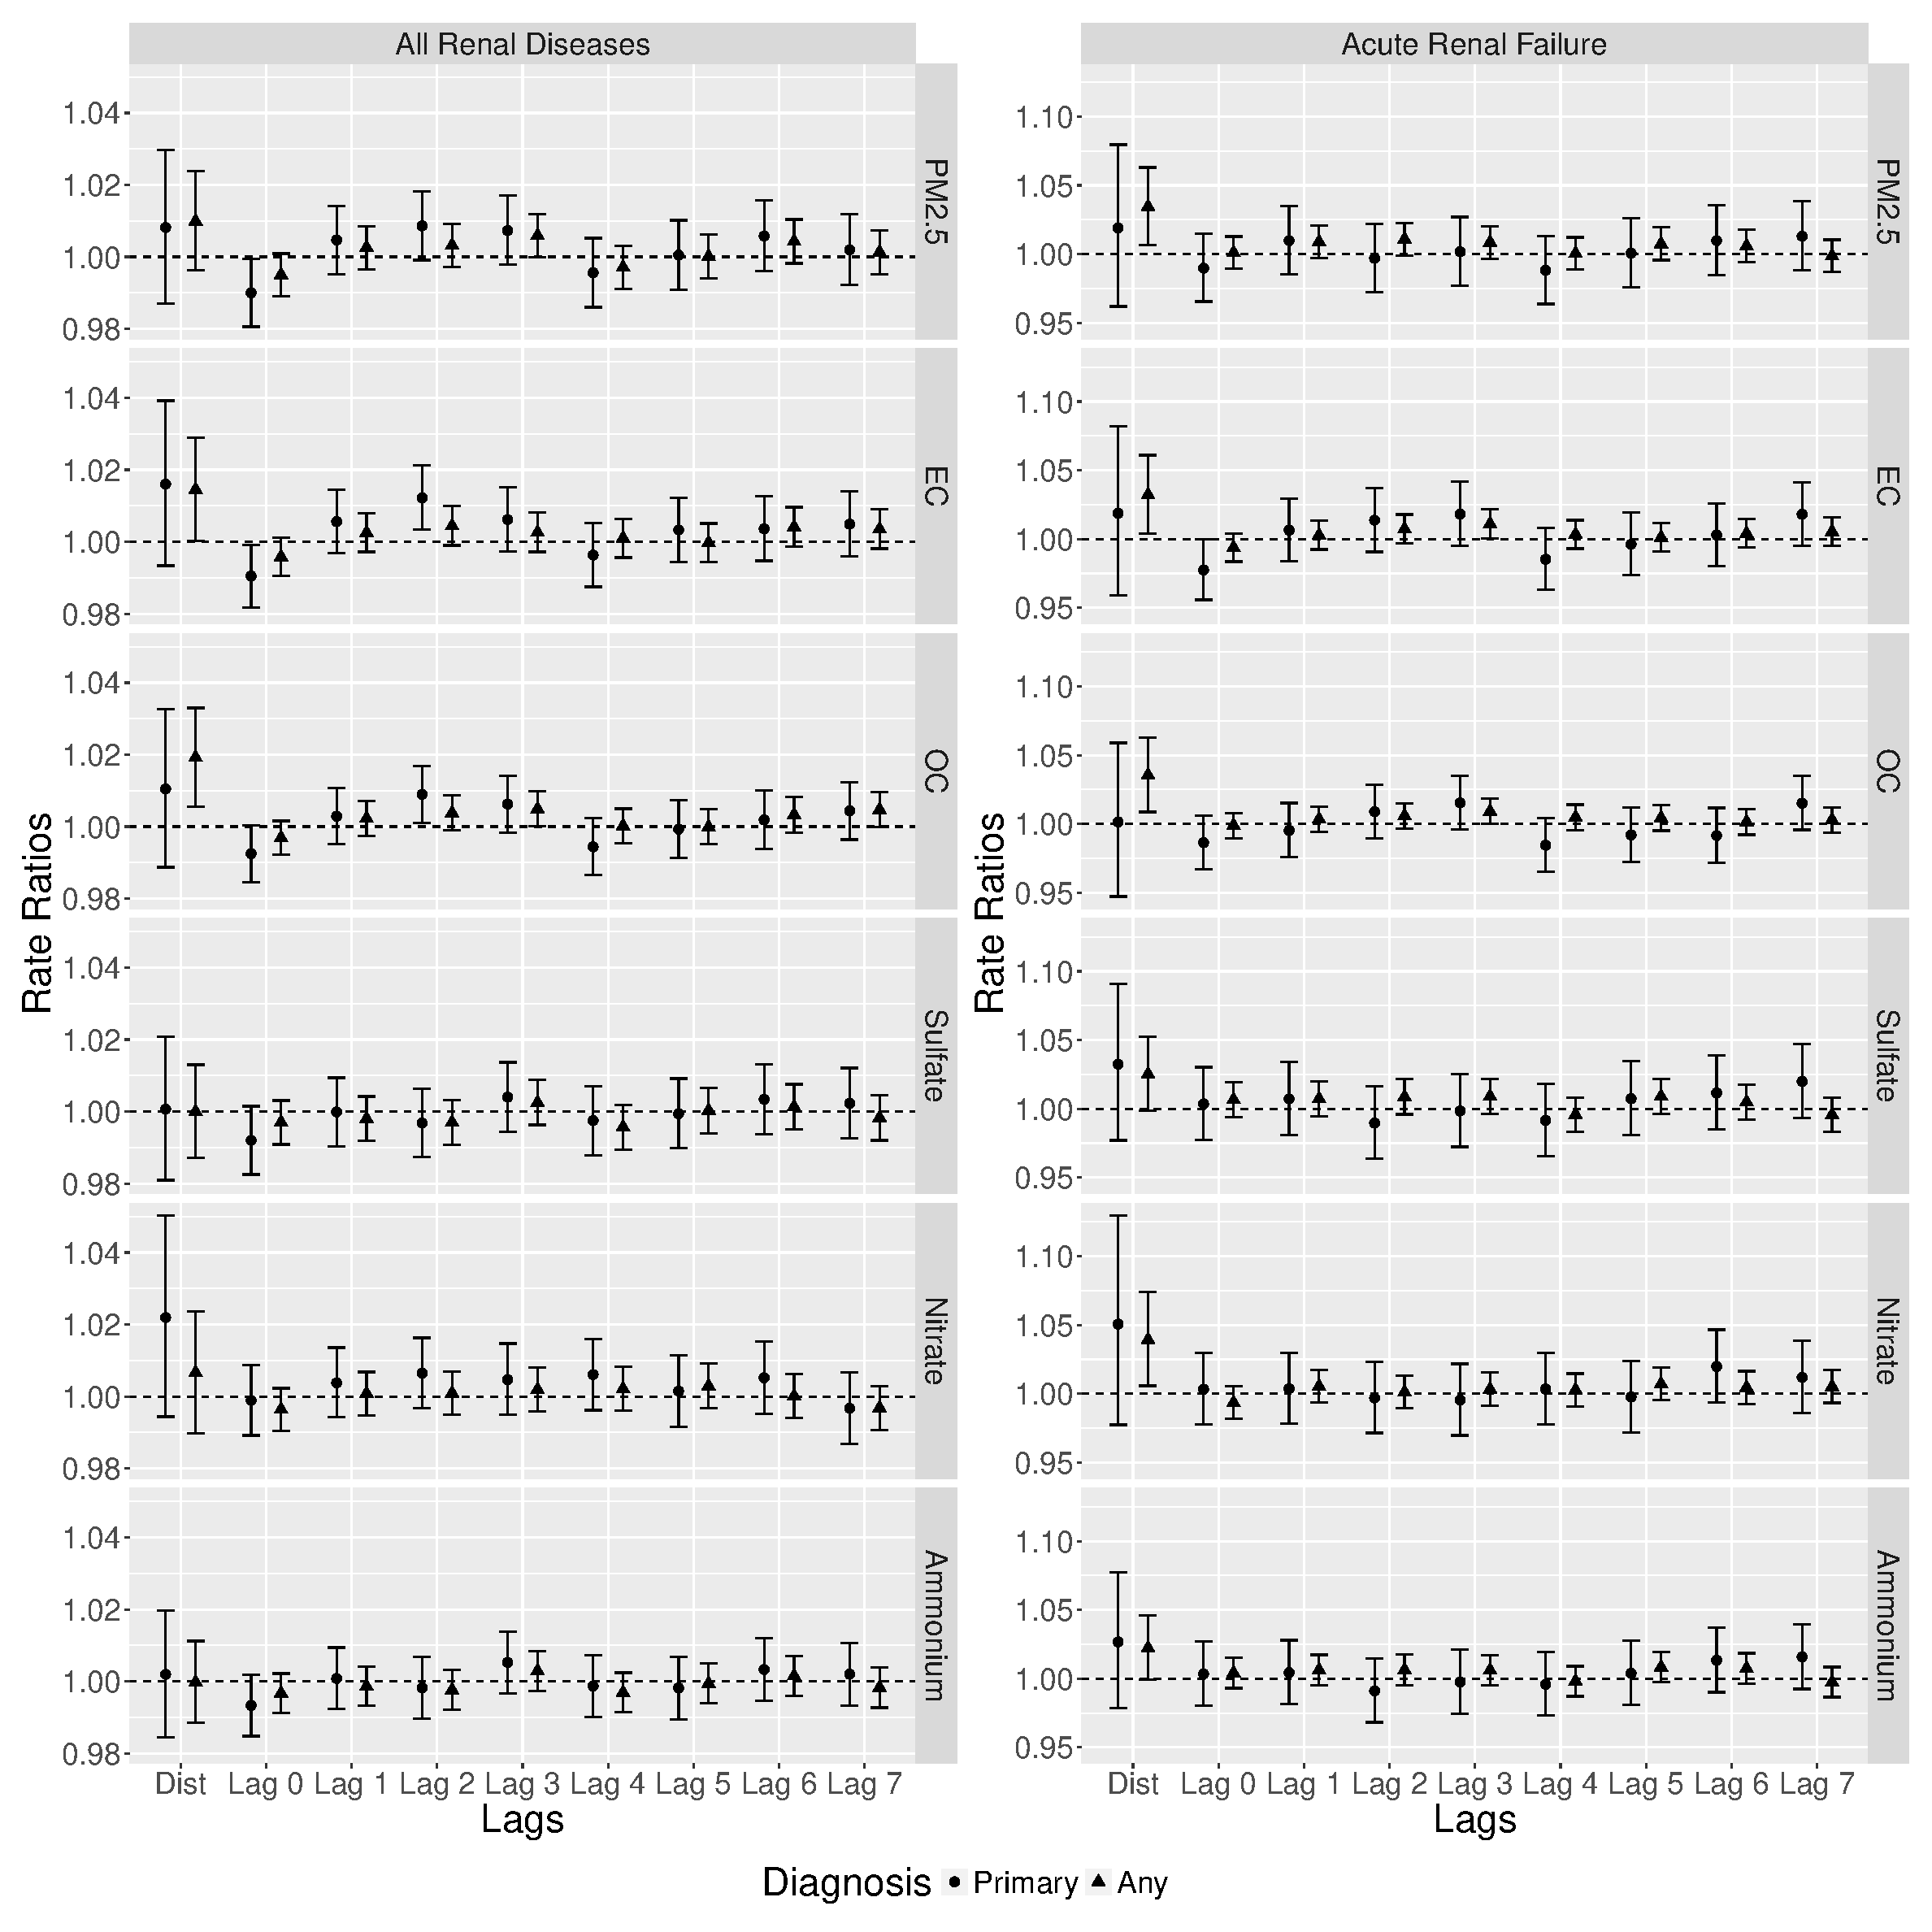
\includegraphics[width=\textwidth]{img/fig3.eps}
\caption{The associations between short-term PM2.5 component exposure and ED visits for renal disease (left panel: all renal diseases; right panel: acute renal failure) with different lag structures and diagnosis types in Atlanta for 2002 -- 2008. The lag structures included 8-day distributed lag (Dist; lag 0 -- 7) and single-day lags (lag 0 to lag 7). Diagnoses included primary (circles) and any diagnoses (triangles).}
\label{fig:renal}
\end{center}
\end{figure}

Figure \ref{fig:renal} shows the associations between the pollutants and outcomes with different lag structures and diagnosis types. For the single-day lags, lag 2 and lag 3 appeared to have the highest positive associations for all renal diseases, and this pattern was not apparent for acute renal failure. Most of the single-day lags for all renal diseases and acute renal failure, however, were not significant at an alpha level of 0.95. In contrast, although the distributed lags had larger confidence intervals (CIs), their associations appeared to be stronger, especially for the ``any diagnoses'' group. For example, 8-day exposure to EC (RR = 1.014, 95\% CI: [1.000, 1.029]) and OC (RR = 1.019, 95\% CI: [1.006, 1.033]) were significantly associated with elevated ED visits for all renal diseases with any diagnoses. 8-day exposure to PM2.5 (RR = 1.035, 95\% CI: [1.007, 1.063]), EC (RR = 1.032, 95\% CI: [1.004, 1.061]), OC (RR = 1.035, 95\% CI: [1.009, 1.063]), and Nitrate (RR = 1.039, 95\% CI: [1.006, 1.074]) were significantly associated with elevated ED visits for acute renal failure with any diagnoses. Overall, in this analysis, we found initial evidence that 8-day PM2.5 component exposure is associated with elevated ED visits for renal disease, especially for acute renal failure, in Atlanta. The effects of other primary diagnoses (\textit{e.g.,} cardiovascular disease, respiratory disease, etc.) on these associations deserve further examinations. 

\subsection{Challenges and Possible Solutions}
One of the major challenges in this study is to effectively calibrate and utilize the low-cost sensors in PM2.5 prediction, especially for those far away from EPA stations. Although two strategies have been proposed, their effects are still unclear. One possible solution for an unfavorable calibration is incorporating some related meteorological variables in the calibration model, since previous studies \citep{Holstius2014, Castell2017} found that the precision of low-cost sensors varies in different temperature and relative humidity conditions. In addition, CTM-simulated PM2.5 components can also be incorporated in the model in order to reflect component-related quality degradation. Another possible solution is to implement appropriate techniques of digital signal processing. For example, Optimal Interpolation (OI) and Ensemble Kalman Filtering (EnKF) have been used to improve the quality of CTM-simulated PM2.5 concentrations by fusing them with regulatory ground measurements \citep{Candiani2013}. The Fourier transform has also been widely applied to reduce the high-frequent noises in the signals \citep{Canales1984}. These techniques may provide new perspectives for handling the measurements of low-cost sensors. 

Another potential challenge in this study is the lack of statistical power in the time-series model due to the limited sample size. Because the measurements of low-cost sensors are available from late 2015, only $\sim$1-year ED visit data can be used in the time-series model. In addition, splitting the ED records by patients' residential ZIP codes will further limit the sample size. One feasible solution is to extend our study domain to more US states in which the low-cost sensor measurements are available. Another possible solution is combining some small ZIP code areas with similar spatiotemporal patterns of PM2.5 pollution. The combination can be conducted by classifying the ZIP code areas in a city according to their features regarding the population and the pollution patterns, using unsupervised or supervised classifiers. 

\subsection{Timeline}
\begin{table}[H]
\small
\begin{center}
\begin{tabular}{|c|c|c|c|c|c|c|c|c|c|c|c|}
\hline
\multicolumn{2}{|c|}{\multirow{2}{*}{Task}} & \multicolumn{2}{|c|}{2018} & \multicolumn{4}{|c|}{2019} & \multicolumn{4}{|c|}{2020} \\
\cline{3-12}
\multicolumn{2}{|c|}{\multirow{2}{*}{}} & Q3 & Q4 & Q1 & Q2 & Q3 & Q4 & Q1 & Q2 & Q3 & Q4 \\
\hline
\multirow{3}{*}{\shortstack{Aim 1:\\AOD gap-filling}} & Data collection & $\times$ & & & & & & & & & \\
\cline{2-12}
\multirow{3}{*}{} & Data analysis & $\times$ & & & & & & & & & \\
\cline{2-12}
\multirow{3}{*}{} & Organization \& publication & $\times$ & & & & & & & & & \\
\hline
\multirow{3}{*}{\shortstack{Aim 2:\\Sensor calibration}} & Data collection & $\times$ & $\times$ & & & & & & & & \\
\cline{2-12}
\multirow{3}{*}{} & Data analysis & $\times$ & $\times$ & $\times$ & $\times$ & & & & & & \\
\cline{2-12}
\multirow{3}{*}{} & Organization \& publication & & & $\times$ & $\times$ & $\times$ & & & & & \\
\hline
\multirow{3}{*}{\shortstack{Aim 3:\\Renal disease}} & Data collection & $\times$ & $\times$ & $\times$ & $\times$ & $\times$ & & & & & \\
\cline{2-12}
\multirow{3}{*}{} & Data analysis & & & & $\times$ & $\times$ & $\times$ & $\times$ & $\times$ & & \\
\cline{2-12}
\multirow{3}{*}{} & Organization \& publication & & & & & & & $\times$ & $\times$ & $\times$ & \\
\hline
\end{tabular}
\end{center}
\end{table}%

\newpage

\phantomsection
\bibliography{bibliography}

\end{document}

%-----------------------------------------------------------------------


